% !TeX root = ../main.tex
% Add the above to each chapter to make compiling the PDF easier in some editors.

\chapter{Hardware Extension}\label{chapter:Hardware Extension}

\section{Components and Design}
The hardware extension used in this project is composed of basically light transmitters that project the NIR light on the patient’s skin and a light sensor that receives the reflected light from the skin and the underlying vessels and tissues and sends it to an android device connected to it via an on-the-go (OTG) cable.

\subsection{On-The-Go Cable}
\subsubsection{Background}
Many of portable devices would benefit from being able to communicate to each other over the USB interface, yet certain aspects of USB make this difficult to achieve such as storage for a large number of device drivers and the ability to source a large current \parencite{otg}.
The OTG (On The Go) specification as a supplement to the USB 2.0 specification was developed to allow a portable device to take on the role of a limited USB host, without the burden of supporting all the functions of a PC.
USB OTG is a known USB standard which was designed to allow peripheral attachment to such items as mice, keyboard, memory sticks etc to small, mobile devices.

In addition to being a fully compliant USB 2.0 peripheral, an On-The-Go device must include other features and characteristics including, but not limited to, full-speed operation as a peripheral as well as a host, targeted Peripheral List, session request protocol and means for communicating messages to the user \parencite{otg}.

\subsubsection{Power Providing Specifications}
When an A-device (hosting device) is providing power on a port, it is required to maintain an output voltage within a specified range on that port, under loads of 0 mA up to the rated per port output of the device’s supply as long as the rated output of the A-device is less than or equal to 100 mA \parencite{otg}.

If the current rating per port of the A-device is greater than 100 mA, then the voltage regulation is required to be between 4.75 V and 5.25 V, and the A-device is required to meet the USB 2.0 specification requirements for power providers \parencite{otg}.


\subsection{Light Emitting Diodes}
\subsubsection{Background}
Light-emitting diode (LED) is a semiconductor device. It consists of a chip of semiconducting material treated to create a structure called a p–n (positive–negative) junction. When connected to a power source, current flows from the p-side or anode to the n-side or cathode, but not in the reverse direction. Charge carriers (electrons and electron holes) flow into the junction from electrodes. When an electron meets a hole, it returns to a lower energy state and releases the energy in the form of a photon (light)\parencite{led}. The specific wavelength or colour emitted by the LED depends on the semiconductor used. The LED light output power ranges from milliwatts to watts. Their typical light beam divergence is approximately $\pm$120 degrees. However, it can be as small as approximately $\pm$5 degrees for the special constructions \parencite{led}. LEDs are very cheap and popular light sources. They are widely used in photomedicine. LEDs convert electrical energy to light with high efficiency and have a long lifetime. They are available in a wide range of wavelengths from UV to IR, including multicolour and white light LEDs. 

\subsubsection{LED Usage in The Project}

According to the previous chapter, the optimal wavelength should be between 800 and 1100 nm, optimally 1100nm. For prototyping purposes, we used a wavelength of 940 nm as it is more available and cheaper in the market. The light beam divergence was estimated optically without taking it into consideration in the research.

To increase the output light power and distribution, a grid of 8 NIR LEDs was used. Each LED is of type SD-AR512C9, voltage 1.2-1.3V, wavelength 940 nm, angle of radiation 60 degrees and current 40mA, connected on parallel with a resistor for each LED. 

The reason why every LED is connected to one separated resistor and not one resistor for all of them is that, when we use one resistor, we have a current limit for the whole LEDs section. After that it's up to each diode to control the current that goes through it. The problem is that real world diodes don't have same characteristics and therefore there's a danger that one diode will start conducting while others won't, which causes one LED to allow more current to flow than it can handle and burn up, eventually then, all other LEDs are going to overheat and burn up because of extra current flowing through them.

A resistor with 100 \si{\ohm} is typically sufficient. As this value should be slightly higher than the minimum resistor value at which the LED has maximum illumination, this can be calculated by Ohm’s low as follows:


\begin{equation}
R= \frac {(V_s - V_{LED})}{I_{LED}} =  \frac {(5-1.2)}{0.04}=95   \si{\ohm}
\end{equation}


where:
\begin{itemize}
  \item $V_S$ is the source voltage, measured in volts ($V$),
  \item $V_{LED}$ is the voltage drop across the LED, measured in volts ($V$),
  \item $I_{LED}$ is the current through the LED, measured in Amperes ($A$), and
  \item $R$ is the resistance, measured in Ohms (\si{\ohm}).
\end{itemize}


To control the illumination of the LEDs so that user can dim them or even turn them off, a stepless variable resistor was added on the whole set of the LEDs so that the current running in the whole LEDs section can be changed and, thus, their brightness. This element is not of much importance because it only adds small value to the overall project, for this reason the resistor's value was estimated based on practical test.


\subsection{NIR Camera}

Cameras are just clever light detectors. Through a sensor, different levels of red, green and blue light are detected and converted into a digital signal, creating an image as the one seen by the human eye. However, infrared and ultraviolet light are present in daylight but cannot be seen by humans. Unlike human eyes, camera sensors can detect NIR light. Infrared light can affect the colour reproduction drastically. To make the image more akin to what humans can see, most cameras are fitted with an IR-Cut filter which only allows visible light to pass through, reflecting unwanted infrared. 

For NIR imaging, exactly the other way around is needed, i.e. passing only NIR light and filtering out any other wavelengths of the EM spectrum. So that any reflections caused by visible light from the epidermis can be out filtered and getting only the image that shows where oxyhaemoglobin has absorbed the NIR light and thus, getting a visual representation of the veins structure. Replacing the IR-Cut filter with IR-Pass filter is sufficient to achieve this goal.

We used a  webcam of type Trust Exis with 640*320 resolution, after removing the IR cut filter and installing a 9mm NIR pass filter, theoretically, any normal web camera should work after replacing the filter.

\begin{figure}[H]
\centering
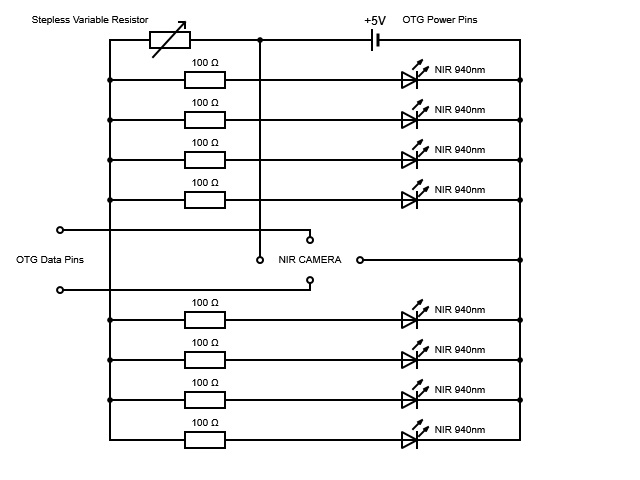
\includegraphics{figures/circuit.jpg}
\caption{The LEDs grid and NIR camera circuit.}\label{fig:circuit}
\end{figure}


\subsection{Power Consumption}
Android devices, especially phones, are powered from batteries which are limited in size and therefore capacity. This implies that a correct energy management is essential in any application running on such devices. Particularly, when the application includes a hardware part powered from the device and thus consumes more energy from the its battery. In this case, energy efficiency of the hardware part is crucial to the application usability or even feasibility at all.

When it comes to USB power, including the OTG, there are two device categories: bus-powered and self-powered. Bus-power is one of the many benefits of a USB design. It allows the device to sustain itself without the need for a bulky power supply either internally or externally because the device draws its power from the bus \parencite{usb}.
There are two classifications for a bus-powered device: high-powered and low powered devices. A low-powered device draws, at most, 100 mA and a high-powered device draws, at most, 500 mA. Anything over 500 mA requires the device to be self-powered \parencite{usb}.

As mentioned in the OTG section, the OTG protocol is fully USB 2.0 compliant and thus, its power providing in the high-powered device mode follows the USB 2.0 specification. Which means OTG cable can provide, at most, 500 mA. Hence, this value is the maximum power consumption limit and cannot be exceeded.

The overall power consumption of the hardware extension can be simply calculated as follows:	Overall Consumption = Consumption of 8 LEDs + Consumption of the NIR camera
	, where the consumption of:
\begin{itemize}
	  \item 8 LEDs = 8 * 40 = 320 mA
	  \item a normal Web camera ranges between 120 and 175 mA
\end{itemize}
Thus the overall consumption is less than 500 mA, one can reduce the LEDs number to 6 in case that the web camera consumes more energy.


\subsection{Heat Emission and Safety}
IR light is generally safe. However, its safety must be reconsidered for such specific usages of it. It is unperceived by any of the human senses, unless from a heat stimulus resulting from high intensity.
In general, IR radiation is classified as nonionizing radiation. Although its energy is deficient for ionizations, it may cause diverse biological effects of thermal origin\parencite{ledEyeSafety}.
Safety of the NIR light should be taken into consideration from two perspectives: eye safety and skin safety.

\subsubsection {Skin Safety Assessment}

The main cause of the potential hazard for NIR light projected on the skin is the heating effect. When NIR light is emitted by an LED without a direct contact, heat is transferred via NIR radiation and absorbed by the skin. However, temperature increase due to the radiated energy has been quantified to be less than 0.5 degrees \parencite{ledSafety}. Which, obviously, can be neglected in this study.

Conducted energy, which is caused by the temperature increase in the semiconductor junction inside the LED, can heat up the skin when there is a direct contact and cause temperature increases of up to 9 degrees for contact durations of 30 mins or more \parencite{ledSafety}.

\subsubsection {Eye Safety Assessment}
The eye lens focusses the light on the retina. Focused light is stronger in terms of irradiance than non-focused light. Hence, injury potential increases with focusing.

In addition, NIR light initiates a very low, or non, visual stimulus. For example, one can look right into an NIR light source without knowing and the defensive mechanisms that typically shields the eye from excessive irradiation are not activated.

However, LEDs have been regarded safe for eye exposure by a number of studies from a radiated energy perspective \parencite{ledEyeSafe1} \parencite{ledEyeSafe2}.
So damage by NIR radiation is caused primarily by the overheating of the irradiated tissue, resulting in the destruction of cells. This can cause, for example, a permanent vision handicap \parencite{ledEyeSafe3} if direct and intense beam was aimed to the eye.
The prototype includes a protective mechanism, so that the user knows that the NIR LEDs should be always kept facing down. An alarm rings if the device is flipped upside down.


\subsubsection{Practical Assessments}
Three practical assessments of the prototype’s temperature increasement and power consumption were performed. The prototype was tested using an old Samsung Galaxy J5 phone. Each assessment was done in the room temperature and for a time duration of 10 minutes and dropped the battery 5\%.

In the first assessment, only the LEDs were left on with full brightness, but the application was not running. It yielded a temperature increase from outside of the device (temperature of one NIR LED) of 3 degrees.

The goal of the second assessment was to test the inner temperature of the prototype. A thermometer was placed inside the prototype. It yielded a temperature increase from inside of the device of 7 degrees which is relatively high.

In the third assessment, the image processing module worked for the whole time period as well as the NIR LEDs in full brightness and the camera. Analogously to the second assessment, a thermometer was also placed inside the prototype. The goal of this assessment is to test the power consumption of the overall system when image processing is on. Result of this assessment was 7 degrees of temperature increasment.

\subsubsection{Conclusion }

\begin{itemize}

\item NIR light is safe for projection on the skin. The main hazard is the heating affect. Which can be neglected in the project setting as the LEDs power is very low. 
\item NIR light can be considered safe for eyes as well, but it is not recommended to aim any kind of directed light beam directly in the eyes.
\item As per the practical assessments, power consumption is reasonable. But the prototype heats up relatively on continuous usage, this can be solved by enhancement of the plastic cover or adding a heat sink.
\item The main power consuming component is the NIR LEDs. Those can be turned off without affecting the imaging quality, given sufficient daylight or at least reflection of it, is available, because the sunlight offers enough amounts of infrared light.

\end{itemize}


\subsection{Device Compatibility}

Unfortunately, having an OTG port is not enough to guaranty that UVC compliant camera will work well under Android. UVC is a standard class for USB video cameras and it will be explained later in a separated section. For reasons related to hardware and chip compatibility, not all android devices can run UVC compliant cameras. 

Moreover, some manufacturers configure their Android image so that devices other than keyboard and mass storage are ignored, and this configuration is hard to detect. 

As no official documentation for the UVC is available, android device compatibility can be checked by installing the app, or any other UVC camera app like CameraFi, and check whether it works. 
A list of compatible and incompatible devices as well as verified cameras can be found in the appendices.


